\documentclass{article}

\usepackage{geometry}
\geometry{a4paper,total={170mm,257mm},left=20mm,top=20mm}

\usepackage{babel}
\usepackage[utf8]{inputenc}

\usepackage{amsmath}
\usepackage{amsthm}
\usepackage{amssymb}
\usepackage[dvipsnames]{xcolor}
\usepackage{fontawesome5}
\usepackage{hyperref}
\usepackage{tikz}
\usepackage{caption}
\usepackage{subcaption}
\hypersetup{linkbordercolor=WildStrawberry, urlbordercolor=RoyalPurple}

\theoremstyle{plain}
\newtheorem{thm}{Theorem}
\newtheorem{lemma}[thm]{Lemma}
\newtheorem{claim}[thm]{Claim}
\newtheorem{observ}[thm]{Observation}

\theoremstyle{plain}
\newtheorem{defn}{Definition}
\newtheorem{problem}{Problem}

\theoremstyle{remark}
\newtheorem*{cor}{Corollary}
\newtheorem*{rem}{Remark}
\newtheorem*{example}{Example}

\title{Notes on connected cuts}
\author{Tomáš Turek}
\date{\today}

\begin{document}
	\maketitle
	
	\tableofcontents
	
	\section{Preliminaries}
	
	We define graph $G = (V,E)$ as usual. Then we talk about edges defined by a cut in the following way. For vertices $S \subseteq V$ we define $E(S, V \setminus S) = \{e \in E \text{ s.t. } |e \cap S| = 1\}$, then the size of a cut is $e(S, V \setminus S) = |E(S, V \setminus S)|$. Also we will talk about the induced subgraphs which will be denoted as $G[S]$ for some vertices $S \subseteq V$. Just to recall that graph is called connected if between every pair of vertices there exists a walk. Also in most cases we will be considering graphs which are connected, but sometimes this is not necessary.
	
	
	\section{Connected cuts definitions}
	
	We will now proceed to some definitions of cuts which are in one way or another connected (meaning that they induce a connected subgraph). We will start simply and build on that.
	
	\subsection{Single cuts}
	
	\begin{defn}[Connected cut]
		For a connected graph $G = (V,E)$ we define connected cut as $S \subseteq V$ for which $G[S]$ is connected. The cut itself is $E(S, V \setminus S)$. Later on we may exchange if we will talk about vertices or edges. Also $(V, E \setminus E(S, V \setminus S))$ is a disconnected graph.
		\label{def-connected-cut}
	\end{defn}
	
	Now we will like to minimize the size of the cut, i.e. the value of $e(S, V \setminus S)$. Also note that the requirement for $G$ being connected is actually not necessary. Sometimes we may even define a connected cut with specific source vertex. This can be formulated by the next definition \ref{def-connected-s-cut}.
	
	\begin{defn}[Connected $s$-cut]
		For a connected graph $G = (V,E)$ and given vertex $s \in V$ we define connected cut as $S \subseteq V$ for which $G[S]$ is connected and also $s \in S$.
		\label{def-connected-s-cut}
	\end{defn}

	This is pretty much the same problem as in previous definition \ref{def-connected-cut}. Note that we would also like to minimize the size of the cut, i.e. $e(S, V \setminus S)$. And if we can solve it for the connected $s$ cut we may also apply it for all $s \in V$ to get the value for general connected cut. Some may already see that the property $G$ being connected is still not necessary.
	
	Some may already know that commonly used cut is for defined source and target distinct vertices. We could also use it in our case and only extend the previous definition by saying that $t \notin S$. It is somewhat tempting to also require that $G[V \setminus S]$ is supposed to be also connected. Therefore we can get the full connected $s-t$ cut.
	
	\begin{defn}[Connected $s-t$ cut]
		For a connected graph $G = (V,E)$ and given two distinct vertices $s, t \in V$ we define connected $s-t$ cut as $S \subseteq V$ for which all following properties hold.
		
		\begin{enumerate}
			\item $s \in S$ and $t \notin S$.
			\item Both $G[S]$ and $G[V \setminus S]$ are connected.
		\end{enumerate}
		\label{def-connected-s-t-cut}
	\end{defn}

	\subsection{Multi commodity cuts}

	Now we can furthermore generalize the notion of connected cuts to multi-way connected cuts.
	
	\begin{defn}[Multi-way connected cut]
		For a connected graph $G = (V,E)$ and pairwise distinct vertices $s_1, s_2, \dots, s_k \in V$ for $k \in \mathbb{N}$ we define connected cut as partition $\mathcal{V} = \{V_1, V_2, \dots, V_k\}$ of vertices (that is $\bigcup_{i = 1, \dots, k} V_i = V$ and for $i \neq j$ $V_i \cap V_j = \emptyset$) such that the following holds:
		
		\begin{enumerate}
			\item $\forall i \in [k]: s_i \in V_i$ and
			\item $\forall i \in [k]: G[V_i]$ is connected.
		\end{enumerate}
	\end{defn}
	
	In this specific definitions we may look at our problem from two perspective. Those two options can be seen by the optimization function for the given problem. Sum version is generally more easy to find the solution, or at least very good approximation. On the other hand optimizing over the max function can be way more tricky. Observe that the sum size is already computed with multi-commodity cut.
	
	\begin{itemize}
		\item \textit{Sum} size as $\sum_{i < j} E(V_i, V_j)$.
		\item \textit{Max} size as $\max_{i \in[k]} E(V_i, V \setminus V_i)$.
	\end{itemize}
	
	 Also we may define \textbf{Flexible multi-way connected cut} as relaxing the previous problem. That is the partition will have $l$ partitions where $0 < l \leq k$ and only $l$ sources are representing their partition. So $\forall i \in [l] , \exists k : s_k \in V_l$.
	
	\subsection{Other cuts}
	
	Now we can even further increase the number of requirements. In this case to the size of $|S|$. Now we will also state what is the optimization function and hence declare a problem.
	
	\begin{problem}[$k$-connected cut]
		For a connected graph $G = (V,E)$ we say $S \subseteq V$ is $k$ connected cut such that all properties hold:
		
		\begin{enumerate}
			\item $|S| = k$.
			\item $G[S]$ is connected.
			\item And we want to minimize $e(S, V \setminus S)$.
		\end{enumerate}
	\end{problem}

	From algorithmic perspective we may also have given source vertex $s \in V$, but as it was stated before we may solve the general case by running $|V|$ times the algorithm for the problem with source.
	
	Note that choosing only two properties from all three can be computed. If we skip the very first one, we may use the result from Garg, which states a linear program having all vertices as such result. Excluding the second one can be also computed via some approximation algorithm for bisection. And Overlooking the last one we just use some search, because we don't care about the size of the result.
	
	\section{Absorptive flow}
	
	We will be now talking about an absorptive flow. Firstly we will state the problem in a common sense. For a graph and a source we get a flow which flows through the graph and every time it goes through a vertex some of the flow gets absorbed into the given vertex. After that we will define a cut which is induced by such flow and later on state an integer program and its linear approximation. Now we properly state the instance.
	
	\begin{defn}[Absorptive flow]
		For a graph $G = (V,E)$ and a vertex $s \in V$, also called the \textit{source}, and for $k \in \mathbb{N}$, such that $|V| \geq k$, we define \textbf{absorptive flow} as a tuple of functions denoted as $(f_V, f_E)$, where $f_V : V \to \mathbb{R}$ and $f_E : E \to \mathbb{R}$. Now these two function must have these properties.
		
		\begin{enumerate}
			\item $\sum_{v \in V} f_V (v) = k$, that is every part of the flow gets absorbed,
			\item $f_V(s) = 1$,
			\item $\forall v \in V : 0 \leq f_V(v) \leq 1$, so all vertices have some limits,
			\item $\sum_{v \in V, (s,v) \in E} f_E(s,v) = k-1$, the flow starts from the source,
			\item $\forall e \in E : 0 \leq f_E(e)$, the flow has to be non-negative, but can be unlimited,
			\item $\forall v \in V \setminus \{s\}: \sum_{u \in V, (u,v) \in E} f_E((u,v)) = \sum_{u \in V, (v,u) \in E} f_E((v,u)) + f_V(v)$, thus the whole flow continue unless part of it is absorbed.
		\end{enumerate}
	\end{defn}
	
	One can already see that it resembles a linear program. Some can expect we would define a size of the flow, but in this special instance we won't be defining it, since the main purpose is to look at the cut, which is defined by the flow. So now we will define the cut.
	
	\subsection{Induced cut by the absorptive flow}
	
	Firstly we will define $S \subseteq V$ as the vertices which have nonzero function $f_V$, that is $\forall v \in S : f_V(s) > 0$. Then the \textbf{induced cut} defined by absorptive flow is defined as $E(S, V \setminus S)$ and its size as $e(S, V \setminus S)$. We will furthermore want to minimize the size of such cut.
	
	So far the only property is that $s \in S$, which can be seen only from the definition. Next observations come from the linear program and its properties.
	
	
	\section{Integer program}
	
	In this section we will establish the linear program which works with this flow and its cut.
	
	\subsection{Variables}
	
	Firstly we declare the variables for edges and for vertices.
	
	$$
	f_v = \left\{\begin{array}{l l}
		1 & \text{if it absorbs the flow} \\
		0 & \text{otherwise}
	\end{array}
	\right.
	$$
	
	$$
	f_{uv} \in [0,k] \text{ is for the amount of flow on the edge } uv.
	$$
	
	$$
	x_{uv} = \left\{\begin{array}{l l}
		1 & \text{if } uv \in E(S, V \setminus S)\\
		0 & \text{otherwise}
	\end{array}
	\right.
	$$
	
	See that these variables arise only from the definition of the problem. There is only change of $f_{uv}$ being limited by $k$, which can be easily observed to be the same.
	
	\subsection{Constraints}
	
	Now we need to state the constraints. Firstly set the connection between the absorbed vertices and the cut.
	
	$$
	\begin{array}{r l}
		x_{uv} \geq f_u - f_v & \forall \{uv\} \in E\\
		x_{uv} \geq f_v - f_u & \forall \{uv\} \in E
	\end{array}
	$$
	
	Which is basically that $x_{uv} \geq |f_u - f_v|$. Next we have to set the flow, so its properties hold.
	
	$$
	\begin{array}{r l}
		\sum_{v \in V, sv \in E} f_{sv} = k-1 \\
		f_s = 1 \\
		\sum_{u \in V, uv \in E} f_{uv} = \sum_{u \in V, vu \in E} f_{vu} + f_v & \forall v \in V, s \neq v \\
		\sum_{u \in V} f_u = k \\
		(k-1)) \cdot f_{v} \geq \sum_{u \in V, \{uv\} \in E} f_{uv} & \forall v \in V \setminus \{s\}
	\end{array}
	$$
	
	The very last constraint is there to ensure some absorption, that is whenever there is some flow to the vertex we must absorb based on the flow and capacity.
	
	\subsection{Optimization function}
	
	Lastly the optimization function will be to minimize the flow throughput and number of cut edges.
	
	$$
	\min \sum_{e \in E} x_e %+ \Delta f_e
	$$
	
	\subsection{The whole formulation}
	
	\begin{equation}
		\begin{array}{r l}
			\min \sum_{e \in E} x_e \\
			x_{uv} \geq f_u - f_v & \forall \{uv\} \in E\\
			x_{uv} \geq f_v - f_u & \forall \{uv\} \in E\\
			\sum_{v \in V, sv \in E} f_{sv} = k-1 \\
			f_s = 1 \\
			\sum_{u \in V, uv \in E} f_{uv} = \sum_{u \in V, vu \in E} f_{vu} + f_v & \forall v \in V, s \neq v \\
			\sum_{u \in V} f_u = k \\
			(k-1) \cdot f_{v} \geq \sum_{u \in V, \{uv\} \in E} f_{uv} & \forall v \in V \setminus \{s\} \\
			f_v \in \{0,1\} & \forall v \in V \\
			f_{uv} \in \mathbb{R}^+ & \forall \{u,v\} \in E \\
			x_{uv} \in \{0,1\} & \forall \{u,v\} \in E
		\end{array}
	\end{equation}
	
	\subsection{Properties}
	
	Lets talk about some crucial properties of this integer program.
	
	\begin{observ}
		Every vertex in the flow absorb.
	\end{observ}

	\begin{proof}
		See that due to the last constraint whenever a flow goes inside the vertex we must set the vertex to absorb some portion of the flow. Exactly 1 in the case of integer program.
	\end{proof}

	\begin{observ}
		$f_V$ defines a connected induced subgraph of $G$.
	\end{observ}

	\begin{proof}
		Since $f_s = 1$ we know that $s$ is inside the $G[S]$. For contradiction assume there is a vertex $v \in S$ which is not connected to the source $s$. Because $f_v = 1$ we must have that there is a flow over this vertex due to the fifth constraint. And since there is a flow to the vertex $v$ which starts in $s$ there is also a walk from $s$ to $v$, therefore no such vertex $v$ exists and all vertices are connected to $s$ and hence they induce connected subgraph.
	\end{proof}

	\begin{observ}
		We have a minimum connected $s$ cut from the optimal integer value of the lp formulation $x^\ast$.
	\end{observ}

	Now it is also a time to talk about integrality, moreover what will happen if we switch to lp relaxation.
	
%	\subsection{Example (which is not correct anymore)}
%	
%	Now consider a simple example of a graph $G$ which is depicted on picture \ref{star-graph}. It is a so called star, where $v$ is the center point with $\Delta$ neighbors. In this special instance $s$ is already provided, now we need to set $k = 2$.
%	
%	\begin{figure}[!ht]\centering
%		\begin{tikzpicture}[main/.style = {draw, circle, inner sep=1.5pt}]
%			\node[main] (s) at (0,0) {$s$};
%			\node[main] (v) at (3,0) {$v$};
%			\node[main] (u) at (6,0) {$u$};
%			\node[main] (3) at (3,3) {};
%			\node[main] (1) at (1,2) {};
%			\node[main] (2) at (2,2.5) {};
%			\node[main] (5) at (5,2) {};
%			\draw[dotted] (3) to (5);
%			
%			\draw (s) -- (v);
%			\draw (v) -- (u);
%			\draw (v) -- (1);
%			\draw (v) -- (2);
%			\draw (v) -- (3);
%			\draw (v) -- (5);
%		\end{tikzpicture}
%		\caption{Star graph $G$ with special vertices $v,s$ and $u$.}
%		\label{star-graph}
%	\end{figure}
%
%	We can easily observe that the optimal solution of such connected $s$ cut is by setting $S = \{s,v\}$ since if $s \in S$ and $G[S]$ has to be connected we can only choose $v$, so that also $|S| = k = 2$. But mainly we are interested in observing how will the integer or linear relaxation of our program work on such instance.
%	
%	\begin{observ}
%		Integer linear program will find the optimal solution.
%	\end{observ}
%
%	\begin{proof}
%		See that $f(s) = 1$ and $f(sv) = 1$ thus $f(v) \geq \frac{1}{\Delta (2-1)} 1 = \frac{1}{\Delta}$. From the property that we have integer variables $f(v)$ must be 1. And hence we absorbed the whole flow and satisfied all constraints. Also the solution can be seen on the picture \ref{star-graph-ilp}.
%	\end{proof}
%
%	\begin{figure}[!ht]\centering
%		\begin{tikzpicture}[main/.style = {draw, circle, inner sep=1.5pt},
%			flow/.style = {Salmon},
%			cut/.style = {dashed, PineGreen}]
%			\node[main,flow] (s) at (0,0) {$1$};
%			\node[main,flow] (v) at (3,0) {$1$};
%			\node[main] (u) at (6,0) {$u$};
%			\node[main] (3) at (3,3) {};
%			\node[main] (1) at (1,2) {};
%			\node[main] (2) at (2,2.5) {};
%			\node[main] (5) at (5,2) {};
%			\draw[dotted] (3) to (5);
%			
%			\draw[flow, ->, thick] (s) -- (v) node[midway, above] {$1$};
%			\draw[cut] (v) -- (u) node[midway, above] {$1$};
%			\draw[cut] (v) -- (1) node[midway, above, right] {$1$};
%			\draw[cut] (v) -- (2) node[midway, above, right] {$1$};
%			\draw[cut] (v) -- (3) node[midway, right] {$1$};
%			\draw[cut] (v) -- (5) node[midway, above left] {$1$};
%		\end{tikzpicture}
%		\caption{Absorbing flow of the integer program.}
%		\label{star-graph-ilp}
%	\end{figure}
%
%	\begin{observ}
%		Linear relaxation will provide a solution with $S = V$ and $x_e > 0$ only for edge $sv$. 
%	\end{observ}
%
%	\begin{proof}
%		The starting point is the same as in previous case, that is $f(s) = 1$ and $f(sv) = 1$. Then we have that $f(v) \geq \frac{1}{\Delta}$. Now suppose that all $N[v] \setminus s$ will have the same value of $f$. So that the cut edge will be only one $sv$.
%		
%		Firstly we must see that this is indeed possible. What if we set $f(vx) = \frac{1}{\Delta}$ for all such neighbors $x \in N[v] \setminus s$, and also $f(x) = \frac{1}{\Delta}$. We have to check if such solution is indeed feasible. Lets sum all
%		
%		$$
%		\sum_{v \in V} f(v) = f(s) + \sum_{v \in V \setminus s} f(v) = 1 + \sum_{v \in V \setminus s} \frac{1}{\Delta} = 1 + (1 + \Delta - 1) \frac{1}{\Delta} = 1 + \frac{\Delta}{\Delta} = 2
%		$$
%		
%		Therefore we have satisfied the constrained of $k$ chosen vertices. Also we can see that the other properties still indeed hold, which are not so hard. For example the flow follow its restrictions. And we have the found the solution given in this observation and shown that it is feasible. The solution is shown on the picture \ref{star-graph-lp}. Now the value of the optimization function is $1 - \frac{1}{\Delta} = \frac{\Delta - 1}{\Delta}$, which $\frac{1}{\Delta}$ times less then the OPT.
%		
%		Lastly we have to see that this is indeed optimal. What can be changed? Only the value of $f(v)$ and flows from vertex $v$. Suppose we would move $\lambda$ back from $u$ to $v$. This will increase $f(v)$ to $\frac{1}{\Delta} + \lambda$ and decreased both $f(u)$ and $f(vu)$ by $\lambda$. This will decrease $x(sv)$ by $\lambda$ and increased $f(vx)$ by $\lambda$ for all neighbors of $v$ without $u,s$. Because for $x(vu)$ we will now have $2 \lambda$ so in total we haven't made a better solution. We would need to split $\lambda$ amongst all $\Delta -2$ such neighbors. But then we will again increase $x(sv)$, so we are in a dead end. All other cases are similar.
%	\end{proof}
%
%	\begin{figure}[!ht]\centering
%		\begin{subfigure}{.4\textwidth}\centering
%			\begin{tikzpicture}[main/.style = {draw, circle, inner sep=1.5pt},
%				flow/.style = {Salmon},
%				cut/.style = {dashed, PineGreen}]
%				\node[main,flow] (s) at (0,0) {$1$};
%				\node[main,flow] (v) at (3,0) {$\frac{1}{\Delta}$};
%				\node[main, flow] (u) at (6,0) {$\frac{1}{\Delta}$};
%				\node[main, flow] (3) at (3,3) {$\frac{1}{\Delta}$};
%				\node[main, flow] (1) at (1,2) {$\frac{1}{\Delta}$};
%				\node[main, flow] (2) at (2,2.5) {$\frac{1}{\Delta}$};
%				\node[main, flow] (5) at (5,2) {$\frac{1}{\Delta}$};
%				\draw[dotted, flow] (3) to (5);
%				
%				\draw[flow, ->, thick] (s) -- (v) node[midway, above] {$1$};
%				\draw[flow, ->, thick] (v) -- (u) node[midway, above] {$\frac{1}{\Delta}$};
%				\draw[flow, ->, thick] (v) -- (1) node[midway, above, right] {$\frac{1}{\Delta}$};
%				\draw[flow, ->, thick] (v) -- (2) node[midway, above, right] {$\frac{1}{\Delta}$};
%				\draw[flow, ->, thick] (v) -- (3) node[midway, right] {$\frac{1}{\Delta}$};
%				\draw[flow, ->, thick] (v) -- (5) node[midway, above left] {$\frac{1}{\Delta}$};
%				\draw[cut, thick] (s) -- (v) node[midway, below] {$\frac{\Delta - 1}{\Delta}$};
%			\end{tikzpicture}
%		\end{subfigure}
%		\begin{subfigure}{.4\textwidth}\centering
%			\begin{tikzpicture}[main/.style = {draw, circle, inner sep=1.5pt},
%				flow/.style = {Salmon},
%				cut/.style = {dashed, PineGreen}]
%				\node[main,flow] (s) at (0,0) {$1$};
%				\node[main,flow] (v) at (3,0) {$\frac{1}{\Delta} + \lambda$};
%				\node[main, flow] (u) at (6,0) {$\frac{1}{\Delta} - \lambda$};
%				\node[main, flow] (3) at (3,3) {$\frac{1}{\Delta}$};
%				\node[main, flow] (1) at (1,2) {$\frac{1}{\Delta}$};
%				\node[main, flow] (2) at (2,2.5) {$\frac{1}{\Delta}$};
%				\node[main, flow] (5) at (5,2) {$\frac{1}{\Delta}$};
%				\draw[dotted, flow] (3) to (5);
%				
%				\draw[flow, ->, thick] (s) -- (v) node[midway, above] {$1$};
%				\draw[flow, ->, thick] (v) -- (u) node[midway, above] {$\frac{1}{\Delta} - \lambda$};
%				\draw[cut, thick] (v) -- (u) node[midway,below] {$2\lambda$};
%				\draw[flow, ->, thick] (v) -- (1) node[midway, above, right] {$\frac{1}{\Delta}$};
%				\draw[flow, ->, thick] (v) -- (2) node[midway, above, right] {$\frac{1}{\Delta}$};
%				\draw[flow, ->, thick] (v) -- (3) node[midway, right] {$\frac{1}{\Delta}$};
%				\draw[flow, ->, thick] (v) -- (5) node[midway, above left] {$\frac{1}{\Delta}$};
%				\draw[cut, thick] (s) -- (v) node[midway, below] {$\frac{\Delta - 1}{\Delta}- \lambda$};
%				\draw[cut, thick] (v) -- (1) node[near end, above, right] {$\lambda$};
%				\draw[cut, thick] (v) -- (2) node[near end, above, right] {$\lambda$};
%				\draw[cut, thick] (v) -- (3) node[near end, right] {$\lambda$};
%				\draw[cut, thick] (v) -- (5) node[near end, above left] {$\lambda$};
%			\end{tikzpicture}
%		\end{subfigure}
%		
%		\caption{Absorbing flow of the linear relaxation.}
%		\label{star-graph-lp}
%	\end{figure}

	\subsection{Consider the distance from source}
	
	In this subsection we will provide even better model, which arises from the previously mentioned one. This time we will also use the notation $d(u,v)$ for shortest path between vertices $u$ and $v$. This is a well known property of graphs, which can be computed in polynomial time (e.g. using Dijsktra's algorithm). Therefore we will increase what we want the vertex absorb by setting the fraction $\frac{1}{k-1}$ to $\frac{1}{k - d(s,u)}$ for every $u$. That is we combine two different metrics of path length. One in terms of standard length and the other of terms flow. The linear program is as follows.
	
	\begin{equation}
		\begin{array}{r l}
			\min \sum_{e \in E} x_e \\
			x_{uv} \geq f_u - f_v & \forall \{uv\} \in E\\
			x_{uv} \geq f_v - f_u & \forall \{uv\} \in E\\
			\sum_{v \in V, sv \in E} f_{sv} = k-1 \\
			f_s = 1 \\
			\sum_{u \in V, uv \in E} f_{uv} = \sum_{u \in V, vu \in E} f_{vu} + f_v & \forall v \in V, s \neq v \\
			\sum_{u \in V} f_u = k \\
			(k-d(s,v)) \cdot f_{v} \geq \sum_{u \in V, \{uv\} \in E} f_{uv} & \forall v \in V \setminus \{s\} \\
			f_v \in \{0,1\} & \forall v \in V \\
			f_{uv} \in \mathbb{R}^+ & \forall \{u,v\} \in E \\
			x_{uv} \in \{0,1\} & \forall \{u,v\} \in E
		\end{array}
	\end{equation}


	\section{Example graphs}
	
	We will be looking at a few graphs and mostly their classes and try to observe some properties.
	
	\subsection{Star graph}
	
	\begin{defn}
		Star graph is a graph with one vertex with degree $\Delta$ and the rest of the vertices have degree 1 and are connected to the main one.
	\end{defn}

	\begin{figure}[!ht]\centering
		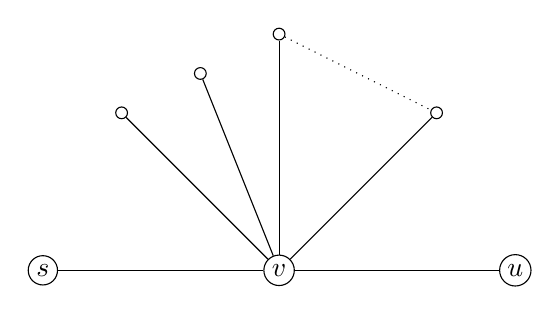
\begin{tikzpicture}[main/.style = {draw, circle, inner sep=1.5pt}]
				\node[main] (s) at (0,0) {$s$};
				\node[main] (v) at (3,0) {$v$};
				\node[main] (u) at (6,0) {$u$};
				\node[main] (3) at (3,3) {};
				\node[main] (1) at (1,2) {};
				\node[main] (2) at (2,2.5) {};
				\node[main] (5) at (5,2) {};
				\draw[dotted] (3) to (5);
				
				\draw (s) -- (v);
				\draw (v) -- (u);
				\draw (v) -- (1);
				\draw (v) -- (2);
				\draw (v) -- (3);
				\draw (v) -- (5);
			\end{tikzpicture}
		\caption{Star graph $G$ with special vertices $v,s$ and $u$.}
		\label{star-graph}
	\end{figure}

	\subsection{Comet graph}
	
	\begin{defn}
		Comet graph contain a star and a tail -- hence the name comet.
	\end{defn}

	\section{Improving the result}
	
	Also there is the fact that we want to have cut edges only when the flow is really low. Otherwise it does not make any sense. So either we may be improving our linear program along the way or just consider this during the approximation.

	\begin{figure}[!ht]\centering
			\begin{tikzpicture}[main/.style = {draw, circle, inner sep=1.5pt}]
					\node[main] (s) at (0,0) {$s$};
					\node[main] (v) at (3,0) {$v$};
					\node[main] (u) at (6,0) {$u$};
					\node[main] (t1) at (7,0) {};
					\node[main] (t2) at (8,0) {};
					\node[main] (te) at (10,0) {};
					\node[main] (3) at (3,3) {};
					\node[main] (1) at (1,2) {};
					\node[main] (2) at (2,2.5) {};
					\node[main] (5) at (5,2) {};
					\draw[dotted] (3) to (5);
					
					\draw (s) -- (v);
					\draw (v) -- (u);
					\draw (v) -- (1);
					\draw (v) -- (2);
					\draw (v) -- (3);
					\draw (v) -- (5);
					\draw (u) -- (t1);
					\draw (t2) -- (t1);
					\draw[dotted] (t2) -- (te);
				\end{tikzpicture}
			\caption{Comet graph $G$.}
			\label{comet-graph}
		\end{figure}
	
	\section{More sources}
	
	Now we will try to use our linear program to also introduce a solution for the multi-commodity case; when we have more sources and all of the parts have to be connected. In this particular case we are considering the case with minimizing the sum.
	
	\begin{equation}
		\begin{array}{r l}
			\min \sum_{e \in E} x_e \\
			x_{uv} \geq \sum_{i \neq j \in [k]} f_u^i - f_v^j & \forall \{uv\} \in E\\
			x_{uv} \geq \sum_{i \neq j \in [k]} f_v^i - f_u^j & \forall \{uv\} \in E\\
			f_{s_i}^i = 1 & \forall i \in [k] \\
			\sum_{u \in V, uv \in E} f_{uv}^i = \sum_{u \in V, vu \in E} f_{vu}^i + f_v^i & \forall v \in V, s \neq v, \forall i \in [k] \\
			\sum_{i \in [k]} f_{u}^i = 1 & \forall u \in V \\
			f_v^i \in \{0,1\} & \forall v \in V, \forall i \in [k] \\
			f_{uv}^i \in \mathbb{R}^+ & \forall \{u,v\} \in E, \forall i \in [k] \\
			x_{uv}^i \in \{0,1\} & \forall \{u,v\} \in E, \forall i \in [k]
		\end{array}
	\end{equation}
	If we would like to minimize the maximal cut, then we would have to change it in a proper way.
	
	\section{NP hardness}
	
	In this section we would like to provide a proof that $k$-connected cut with weights is NP complete problem. One can already see whats the definition of wights, but we will still clarify this. In $k$-connected cut we will also have a wight function $w : E \to \mathbb{R}^+_0$ and we want to minimize the sum of weights in the edge cut. That is the non-weighted version has constant  weight function equal to 1.
	
	Now we will state a well known NP complete problem: \textit{Knapsack}. That is we have $n$ items which we can enumerate with the set $[n] = \{1, 2, \dots, n\}$. Then we have weights of the items: $w [n] \to \mathbb{R}^+$ and also values: $v : [n] \to \mathbb{R}^+$. Lastly we also have a capacity $k$. The goal is to pick a subset $A \subseteq [n]$ such that $\sum_{a \in A} w(a) \leq k$ and the value $\sum_{a \in A} v(a)$ is maximized.
	
	Lets have an instance of knapsack problem; that is $(n, v, w, k)$ and we will create a graph where $G = (V,E)$ where $k$-connected weighted cut will correspond to the solution of knapsack problem.
	
	\subsection{Reduction}
	
	Firstly we will introduce a source vertex $s$. Then we will add $k - 1$ vertices which we will call null-vertices. These will be connected to $s$ and the edges will have weight 0. Then for every item in $[n]$ we will create a clique $K_{w(n)}$; that is the size os equal to the weight og an item. We will connect each clique to the source by one edge with the weight equal to the value of an item. Also the edges inside each clique will be equal to the value of the item.
	
	Note that we assume the weights and values are in $\mathbb{N}$. Which can be for numbers in $\mathbb{Q}$ done easily by scaling the numbers.
	
	\begin{observ}
		For a solution $S \subseteq V$ of $k$-connected weighted cut when a vertex $v$ from a clique $K$ is inside $S$ then $K \subseteq S$.
	\end{observ}

	\begin{proof}
		Suppose that is not the case and there is $u \in K$ such that $u \notin S$. Hence the cut inside the clique adds $(w(a)-1) \cdot v(a)$ which is clearly larger or equal then $v(a)$. Because if $w(a) = 1$ then it does not make sense, because if one vertex is chosen, then all are; since there is only one. So we would get equal or better solution by choosing null-vertices instead.
	\end{proof}

	If we assume the weights are at least 3, then it is strictly better.
	
	\begin{observ}
		If at least two items can be chosen, then $s$ is inside best solution.
	\end{observ}

	\begin{proof}
		This property arises from the fact that $s$ connects all parts together.
	\end{proof}

	Hence when we compute the $k$-connected weighted cut we obtain a set $S$ where $s \in S$ and for some indices $i_1, i_2, \dots, i_m$ the cliques $K_{i_1}, K_{i_2}, \dots, K_{i_m} \subseteq S$ and also some null-vertices are in $S$ as well. These cliques correspond to the chosen elements of the knapsack problem.
	
	\begin{thm}
		This solution of the knapsack problem is optimal.
	\end{thm}

	\begin{proof}
		Imagine we would have a better solution. Firstly consider case where an element $a$ can be added to the solution. This would mean that we have some unused capacity. Therefore in our cut we have used null vertices and we could instead use corresponding clique. But that would get us a better solution which is a contradiction. Hence in some sense it is at least good as greedily creating maximal set.
		
		Lets now suppose that there are items $a_1, a_2, \dots a_l \in S$ and $b_1, b_2, \dots b_m \notin S$ which can be exchanged for a better solution. In the cut we would have capacity for doing so. Also $b$'s add $\sum v(b)$ to the cut cost whereas the $a$'s would add $\sum v(a)$. But since $\sum v(b) > \sum v(a)$ it means that we would get a better cut, which is a contradiction with the optimality of the cut.
	\end{proof}

	\begin{observ}
		The reduction is in polynomial time.
	\end{observ}

	\begin{proof}
		We create 1 source vertex, $O(k)$ null vertices and $O(\sum_{a \in A} w(a))$ vertices for cliques. Then we add $O(k)$ edges for null vertices, $O(|A|)$ connections to the cliques and $O(\sum_{a \in A} w^2(a)$ edges inside each clique. Hence all together it is $O(W^2 + k)$ where $W = \sum_{a \in A} w(a)$.
	\end{proof}
	
	\section{Links}
	
	Here I am keeping some useful links.
	
	\begin{enumerate}
		\item \href{https://www.semanticscholar.org/paper/Approximating-unique-games-Gupta-Talwar/a90ecfd407e1730c9039fdc46e7efefcc46dcfda}{Approximating unique games}
		\item \href{https://www.khoury.northeastern.edu/home/austin/papers/bisection.pdf}{Minimum Bisection}
		\item \href{https://epubs.siam.org/doi/abs/10.1137/120873996}{Min max and small set expansion}
		\item \href{https://link.springer.com/article/10.1007/s00453-021-00870-3}{Approximation algorithms for maximally balanced connected graph partition}
		\item \href{https://www.sciencedirect.com/science/article/pii/S0304397515009378}{On size-constrained minimum s–t cut problems and size-constrained dense subgraph problems}
		\item \href{https://link.springer.com/article/10.1007/s10107-023-01987-9}{On the minimum $s-t$ cut problem with budget constraints}
		\item \href{https://drops.dagstuhl.de/entities/document/10.4230/LIPIcs.ESA.2021.26}{Balanced Crown Decomposition for Connectivity Constraints}
	\end{enumerate}
	
\end{document}